\clearpage
\section{원 입력의 실제 계산과 독립 검토}

\subsection{계산식에서 포함 구간까지}

\texttt{mixed\_response\_application.py}는 원 PHYS14의 exact Fraction
산술과 256-bit 바깥쪽 dyadic 반올림을 사용한다. 원 source와 carry의
signed value, gradient, Hessian, $U,V,W$를 읽어 유한 구간 연산만
실행한다. 새 atomic source 평가, 비선형 물리 root solve, 물리 history
재생 횟수는 모두 0이다. 실제 처리 순서는 다음과 같다.

\begin{enumerate}
\item 원 first-half/Full의 $U,V,W$, carried second-half의 $U,V,W$와
PHYS16의 $d,s$, PHYS17의 $d_\lambda,d_b,s_\lambda,s_b$를 결박한다.
각 도함수는 같은 $\alpha$, COMMON, 전역 매개변수를 뜻한다.
\item 35개 광자 좌표에 $(v,\partial_\lambda v,\partial_bv,
\partial_{\lambda b}v)$의 mixed jet을 놓는다. 첫 stage의 incoming,
absorbed, outgoing과 두 번째 stage의 incoming, absorbed, outgoing,
guard에 보존된 포함을 교차한다. 실제 scalar 교차 수는 800개다.
\item 두 번째 stage 식으로 $s_{\lambda b}$를 포함하고 원 $W-W_1$
포함과 교차한다. 같은 작은 $s_{\lambda b}$가 기체 source 이동과
광자 흡수율 차의 mixed product에 함께 들어간다.
\item HH 기울기와 nonphoto source의 밀도 차는 PHYS17의 정확한 He
projector 미분으로 구성한다. 원 signed Hessian의 차를 사용하여
$C^2$에서 닫히는 모든 source 항을 평가한다.
\item 직접 mixed implicit 식과 상관된 mixed residual 식을 각각
같은 Full $C,B,q,S$에 넣는다. 이 두 포함과 원 $W_2-W_F$를 교차한다.
\item $\Pi_F>0$에서 정확한 유한 온도 mixed quotient를 적용하고,
같은 역연산자와 온도 covector로 각 강제항과 묶음별 기여를 읽는다.
\end{enumerate}

역 포함의 핵심을 명시하면 $E=I-CJ_F$, $|E|\le B$,
$\|E\|_S\le q<1$이고, $J_Fz=f$에 대해
\[
a=(I-B)^{-1}|Cf|,\qquad
z\in Cf+[-Ba,Ba]
\]
를 사용한다. $(I-B)a=|Cf|$는 유리수 선형 연산으로 확인한다.
이어 $z=Cf+Ez$의 signed 교차로 포함을 좁힌다.
상쇄를 보존한 우변은 각 경로를 별개로 크게 포함한 뒤 빼는 폭을 줄인다.
정의역과 original $B,q,S$의 조건은 그대로다.

직접식의 온도 포함은
$[-3.819468564815,-0.8533085984866]\times10^{-12}\ {\rm K}$이고,
원 mixed 응답을 뺀 포함은
$[-6.545446896199,0.6907235324700]\times10^{-12}\ {\rm K}$다.
상관식은 원 subtraction보다 폭을 약 13.16배, 직접식보다 약 5.40배
줄인다. 구간 폭의 감소와 부호 판별은 같은 물리계에서 얻은 결과다.

\subsection{혼합 작용의 공통 전달}

\begin{figure}[H]
\centering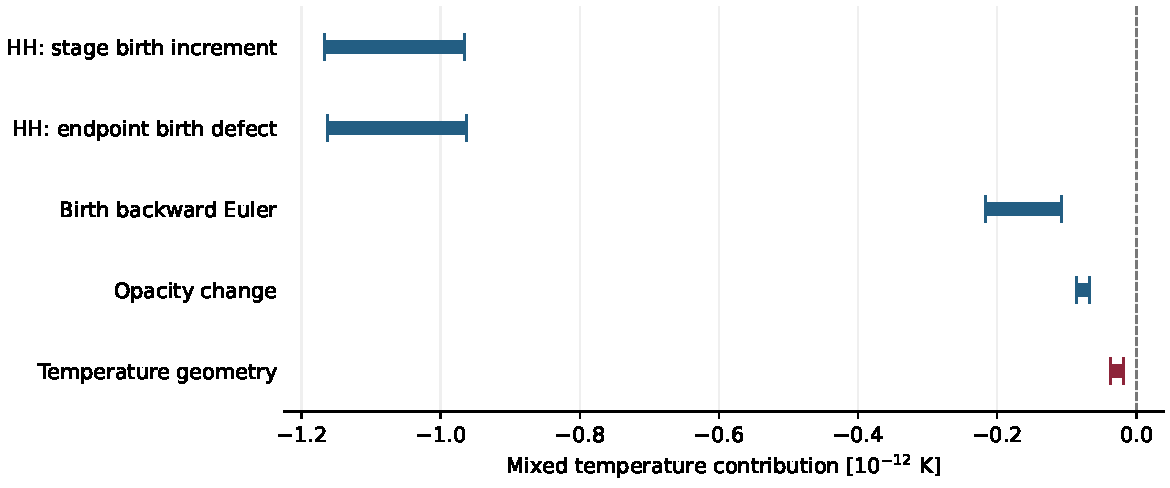
\includegraphics[width=0.96\linewidth]{figures/mixed_mechanism.pdf}
\caption{음의 혼합 응답을 결정하는 주요 항. HH와 광자 강제항은 같은
Full 역연산자와 온도 covector로 전달했다. 온도 geometry는 유한
quotient에서 별도로 더해지는 항이다. 광자 seven-sector의 일부 mixed
부호는 0을 포함하지만, 공통 광자 묶음은 음수로 포함된다.}
\end{figure}

두 HH 기울기 항은 각각 약 $10^{-12}\ {\rm K}$ 규모다. 명시적으로 분리한 다섯 HH
gradient 항을 원 우변에서 먼저 더한 후 공통 inverse로 전달하면
$[-2.329668009361,-1.928397581837]\times10^{-12}\ {\rm K}$다.
광자 일곱 항을 같은 방식으로 묶은 값은
$[-3.024678223968,-1.735793802686]\times10^{-13}\ {\rm K}$다.
나머지 기체와 endpoint 항의 합은
$[2.819648272515,11.40914739344]\times10^{-16}\ {\rm K}$로 작다.
온도 분수에서 추가되는 기하 항은
$[-3.666218766444,-1.794167181955]\times10^{-14}\ {\rm K}$다.

성분별 또는 묶음별 포함을 다시 합한 구간의 폭은 전체 우변을 한 번에
전달한 구간보다 조금 클 수 있다. 그 차이는 같은 참값에 대한 서로 다른
구간 표현에서 생긴다. 최종 채택값은 전체 상관 우변의 포함이다.
가장 큰 세 가지 성분별 폭은 stage HH gradient, endpoint HH gradient,
birth backward Euler이고 각각 약 $2.015\times10^{-13}$,
$1.994\times10^{-13}$, $1.091\times10^{-13}\ {\rm K}$다.
endpoint source Hessian 공간차 항의 폭은 약
$4.576\times10^{-16}\ {\rm K}$에 머문다.

\subsection{실행 기록과 교정}

주 application의 성공 실행은 wall $0.967359\ {\rm s}$,
CPU $0.930019\ {\rm s}$, peak RSS $43744\ {\rm KiB}$였다.
원 구간의 기여 묶음과 유한 사각형 귀결을 계산한 readout은
wall $0.114273\ {\rm s}$, CPU $0.070526\ {\rm s}$,
peak RSS $17568\ {\rm KiB}$였다. 두 결과는 별도 디렉터리에 동결했다.

첫 application은 guard를 숫자 인덱스로 읽어 \texttt{KeyError}가 났다.
원 guard의 이름은 \texttt{number}, \texttt{energy\_eV\_per\_H}였으므로
해당 필드 접근만 교정하여 다음 실행을 완료했다. 원 실패 source와
로그, 실행 자원 기록은 그대로 보존했다. 이는 자료 schema 접근의
구현 오류이며 원 물리 입력의 변경을 수반하지 않는다.

\subsection{실제 Wolfram과 xAct 검산}

Wolfram Language 15.0.1 Linux kernel에서 공식 xAct archive를
받아 SHA-256을 대조하고 xTensor 1.3.0을 실제로 불러왔다.
추상 지수 표준화에는 xPerm 1.2.4의 Wolfram Language group
algorithm을 사용했다. \texttt{\$xpermQ=False}는 tensor 정의와
\texttt{ToCanonical} 호출 전에 설정했다.

추상 지수 검산 7개는 mixed defect cancellation, bilinear 차,
균형 bilinear 차, stage Hessian 수축 차, Hessian mixed 대칭,
공통 adjoint, adjoint Hessian 대칭이며 모두 정확히 0이었다.
스칼라와 행렬 성분 14개도 모두 0이었다. 여기에 일반 $C^2$ mixed
chain rule, source mixed composition, HI Hessian 분모 차,
birth gradient 분모 차, mixed jet 곱과 역수, 유한 온도 quotient,
두 슬롯 비가환 remap의 seven-sector mixed 미분이 포함된다.
상징 연산 시간은 $1.216823\ {\rm s}$였다.

실행 서비스는 임의의 함수 기호 \texttt{HH18}, \texttt{B18}에 대해
\texttt{Symbol::undefined2} 진단을 출력했다. 두 기호는 일반 함수의
형식 미분을 비교하기 위해 의도적으로 미지정한 함수이며, 해당 도함수를
유지한 양변 차이가 0으로 단순화됐다. 원 진단과 실제 출력은 보존했다.
Wolfram context의 최초 내부 오류도 재시도 후 정상 응답한 환경 기록으로
구분한다. 35개 원 물리 슬롯의 수치 포함은 앞의 application이 담당한다.

\subsection{독립 검토의 판정}

별도 검토자는 후보 application 및 PHYS14 프로그램을 import하지 않고,
원 입력에 대한 자체 exact interval 산술과 Cramer determinant 방식의
선형 역 인증을 사용했다. 독립 arithmetic 22개 묶음이 모두 통과했다.
nilpotent polynomial 계수 합성으로 일곱 광자 항의
$7\times35\times4=980$개 성분을 각각 계산했으며,
모두 후보 포함 안에 들어갔다.

검토는 원 input identity, $U/V/W$와 parameter slot, Full birth의 2배
인수, 직접/상관 혼합 우변, 원 $C^2$ density bridge, stage mixed
increment, 유한 온도 분수, 공통 inverse의 세 기여 묶음을 포함한다.
mixed number/energy ledger는 두 guard를 유지한 잔차의 0 포함을
확인했다. 현재 수치의 음의 margin도 독립 유리수 계산과 일치한다.

독립 검사 첫 시도는 바깥쪽으로 저장된 decimal prior를 유리수
singleton으로 가정한 checker의 표현 오류를 발견했다. 실제 표현인
바깥쪽 구간 포함으로 판정식을 교정하여 다음 실행에서 22/22를
통과했다. 이 과정에서 생산 코드와 수치 결과는 바뀌지 않았다.
이론 정리 8개와 따름정리 4개는 이 범위에서 \texttt{PROMOTE\_SCOPED}로
채택한다. 남은 과학적 차단 사유는 없다. 실제 최종 해시와 채택은
\nolinkurl{review/INDEPENDENT_REVIEW.json},
\nolinkurl{review/DECISION.json}에 기록한다.


\section{문헌의 결과와 현재 구성의 관계}

SciSpace와 Exa로 2차 implicit sensitivity와 공통 관측량 adjoint를
검색하고 원문을 대조했다. Safiran--Lotz--Naumann의 정리 4.3은
parameterized nonlinear system의 2차 tangent를 원 state Jacobian과
Hessian 수축의 선형식으로 구성한다. 매개변수 seed를 서로 다른 두
좌표 방향으로 놓으면 이번 $J_FW_F=-\mathcal B(g_F;U_F,V_F)$와
일치한다. 이 implicit 관계는 원 $C^2$ 식에서 유도된다. 반복 Newton
알고리즘 자체를 두 번 AD하는 별도 구성의 미분 차수와 구별하여
적용했다.\cite{SafiranLotzNaumann2015}

Lewis의 정리 2.2와 식 (7)--(14)는 $C^2$ state equation과 관측량,
가역 state derivative 아래 tangent와 adjoint로 reduced Hessian을
구성한다. Pacaud 등의 2차 adjoint 구현도 Jacobian/transpose solve와
Hessian의 두 방향 수축을 결합한다. 이 구조는 하나의 Full inverse와
온도 covector로 현재 mixed forcing을 읽는 데 대응한다.
\cite{Lewis1997,PacaudEtAl2022}

Xue의 incremental state/adjoint 관계는 2차 implicit 검산의 현대적
비교 자료다. 현재의 전체 parameter-box 부호와 바깥쪽 오차 포함은
이 연구의 원 signed 자료 및 exact interval 연산에서 직접 얻었다.
\cite{Xue2025}

현재 구성은 표준 미분식을 WU088\_HH의 density bridge, 작은 결함,
같은 매개변수의 광자 chronology와 유한 온도에 연결한다.
원문 적용 위치와 접근 기록은
\nolinkurl{literature/LITERATURE_REVIEW_KO.md}에 있다.
